% !TEX TS-program = LuaLaTeX
\documentclass[11pt,compress,xcolor=x11names,UTF8]{beamer}
\usetheme{Boadilla}
\usecolortheme{seahorse}
\useinnertheme[shadow]{rounded}  
\useoutertheme[subsection=false]{smoothbars}
\usecolortheme{spruce}
\usecolortheme[named=SpringGreen4]{structure}
\usefonttheme{structurebold}
\useinnertheme{circles}
\usecolortheme{rose}
\usepackage{pifont}
\usepackage{academicons}
\usepackage{fontawesome}
\usepackage{iitem}
\setbeamertemplate{itemize item}{\ding{108}}
\setbeamertemplate{itemize subitem}{\ding{109}}
\setbeamertemplate{navigation symbols}{}
\setbeamercovered{transparent}  
\renewcommand\appendixname{附录}
\renewcommand\abstractname{摘要}
\graphicspath{{figure/}} % 图片路径
\usepackage{calligra} % Thank you
\usepackage{ctex} % 加入中文
%\setCJKsansfont{Noto Sans CJK SC}
\setsansfont{Lato} % Lato Roboto Fira Sans
\usepackage{makecell}
\newcommand{\tabincell}[2]{\begin{tabular}{@{}#1@{}}#2\end{tabular}}
\usepackage{url}					
\usepackage{natbib} % 参考文献
%\title[Spatial Generalized Linear Mixed Models]{Spatial Generalized Linear Mixed Models with Application to Prevalence Mapping}
\title{TTS Measurement in container 1 }
%\subtitle{奖助金申请答辩}
\author[Rong. Zhao]{Email:zhaor25@mail2.sysu.edu.cn \and  } % \\ 专业:统计学 \\ 方向:数据分析与统计计算
\institute[Sun Yat-Sen University]{School of Physics\and } % 理学院\\
\date[\today]{
\includegraphics[width=.5\textwidth]{logo}}

\begin{document}

\maketitle

%\begin{frame}{Outline}
%\tableofcontents
%\end{frame}

\section{current results}

%\subsection{研究意义}

\begin{frame}{Trigger Time and Signal Time}
Below is a typical \alert{trigger time --- signal time} correlation histogram.
%\textsf{例} \textbf{例}  \textit{例} 
% \texttt{例}  % 调出仿宋字体了
\begin{figure}
\centering
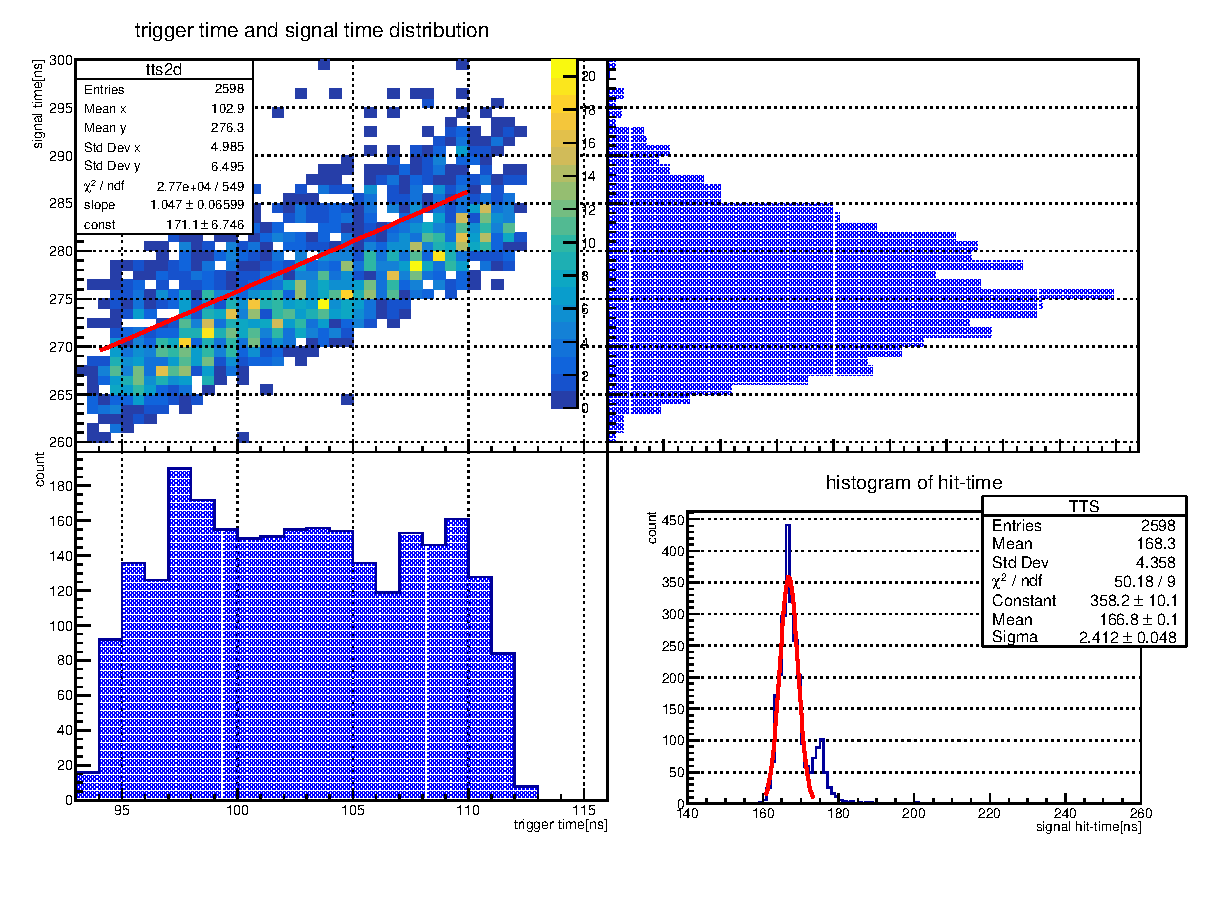
\includegraphics[width=0.78\textwidth]{typical_hittime} % 单图
\end{figure}

\end{frame}
\begin{frame}{discuss about the results}
The data of this plot is from container 1, mass274, drawer 113, SN=EA1578, one of the reference tubes.\\
"time-amplitude" correction is applied.
\vspace{.5cm}
\hrule{}
\hrule{}
\vspace{.5cm}

We can see from the above figure that:
\begin{itemize}
\item The PMT signal time is proportional to trigger time as we expected.
\item Trigger time follow a uniform distribution 
\item PMT signal time, which is the convolution of PMT-TTS and system response, is gaussian like.
\item In the 2-D histogram, two adjoining linear bands exist corrsponding to the small peak in the "hit-time" histogram.
\end{itemize}
\end{frame}

%\section{学术活动}
%%%%%%%%%%%%%%%%%%%%%%%%%%%%%%%%%%%%%%%%%%%%%%%%%%%%%%%%%%%%%%%%%%%%
\begin{frame}{same PMT another drawer}
	\alert{“but when the same PMT was tested in another drawer”, we see only one peak in the hit-time distribution histogram.}
\begin{figure}
\centering
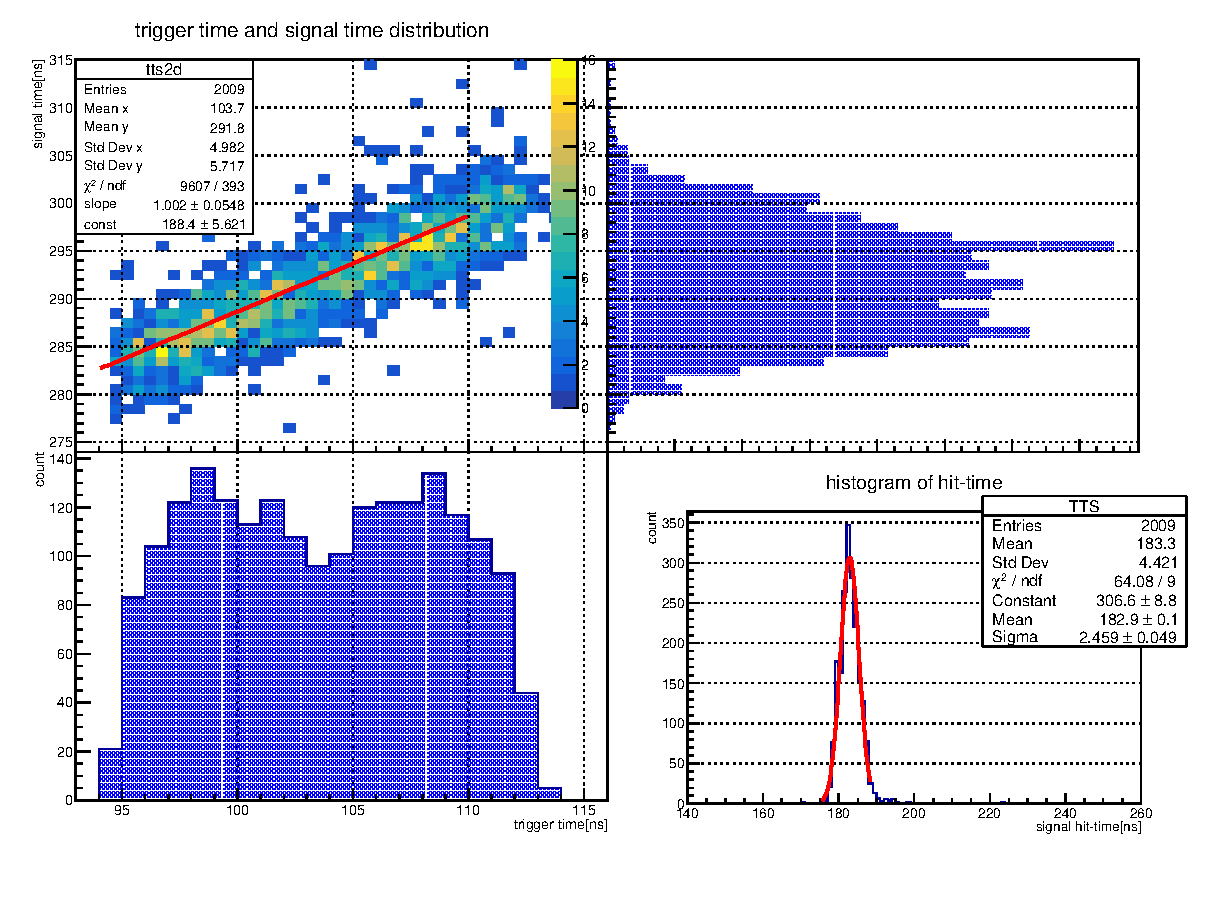
\includegraphics[width=0.74\textwidth]{ea1578-283} % 单图
\end{figure}
\end{frame}
\begin{frame}{discuss about the results}
The data of this plot is from container 1, mass283, SN=EA1578,drawer124.\\
\vspace{.5cm}
\hrule{}
\hrule{}
\vspace{.5cm}

The hit-time performance of EA1578 is quite different in two drawers, and then I guess the small peak in the "hit-time" histogram may not caused by PMT itself.
\vspace{.5cm}
\hrule{}
\hrule{}
\vspace{.5cm}
Then I focus on the two drawers 124 and 113 , and extract the data when another referencre tube "EA0419" was tested in these drawers.
\end{frame}
%%%%%%%%%%%%%%%%%%%%%%%%%%%%%%%%%%%%%%%%%%%%%%%%%%%%%%%%%%%%%%%%
\begin{frame}{EA0419}
when EA0419 was tested in drawer 113 and mass 282, the "small peak" appeared again.
\begin{figure}
\centering
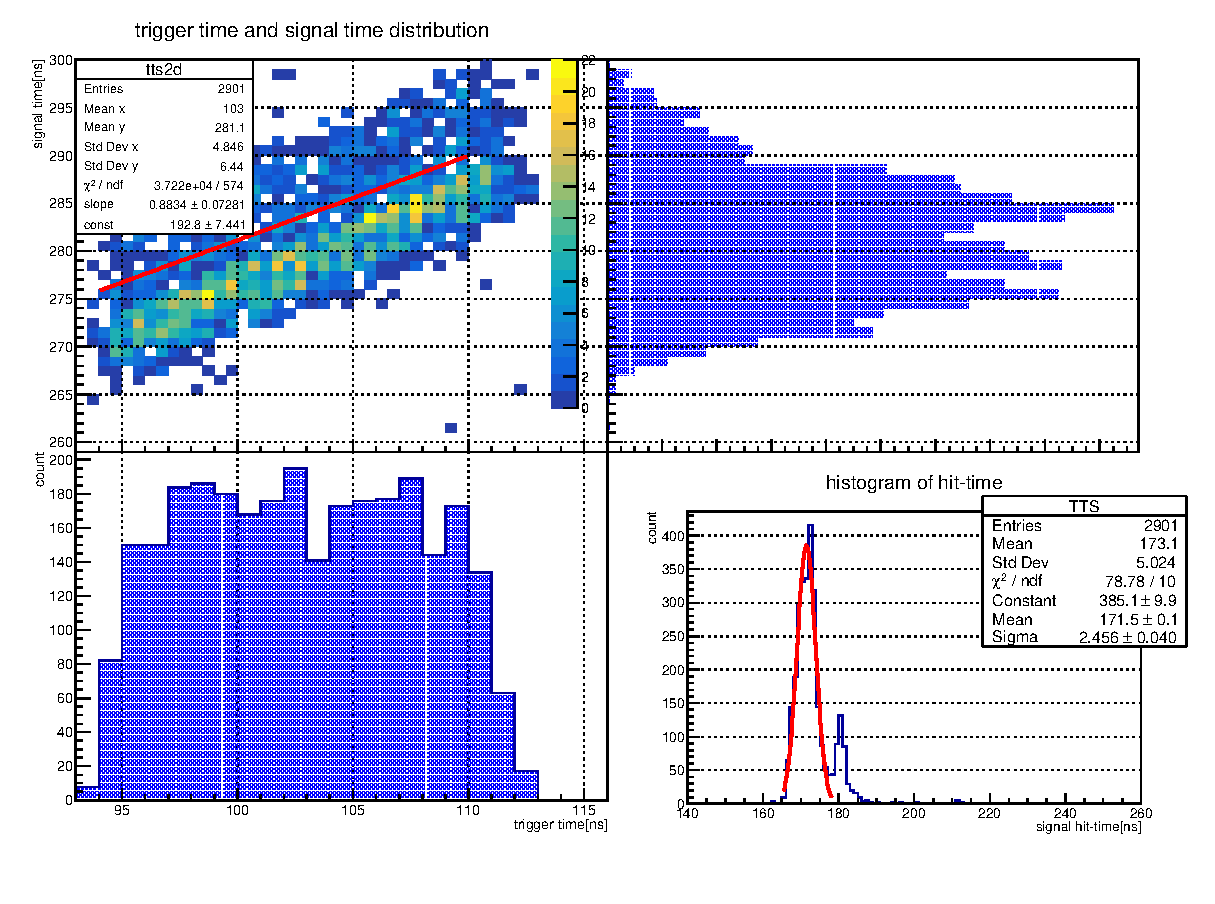
\includegraphics[width=0.74\textwidth]{ea0419-282} % 单图
\end{figure}
\end{frame}
\begin{frame}{EA0419}
when EA0419 was tested in drawer 124 and mass 273, the "small peak" disappeared.
\begin{figure}
\centering
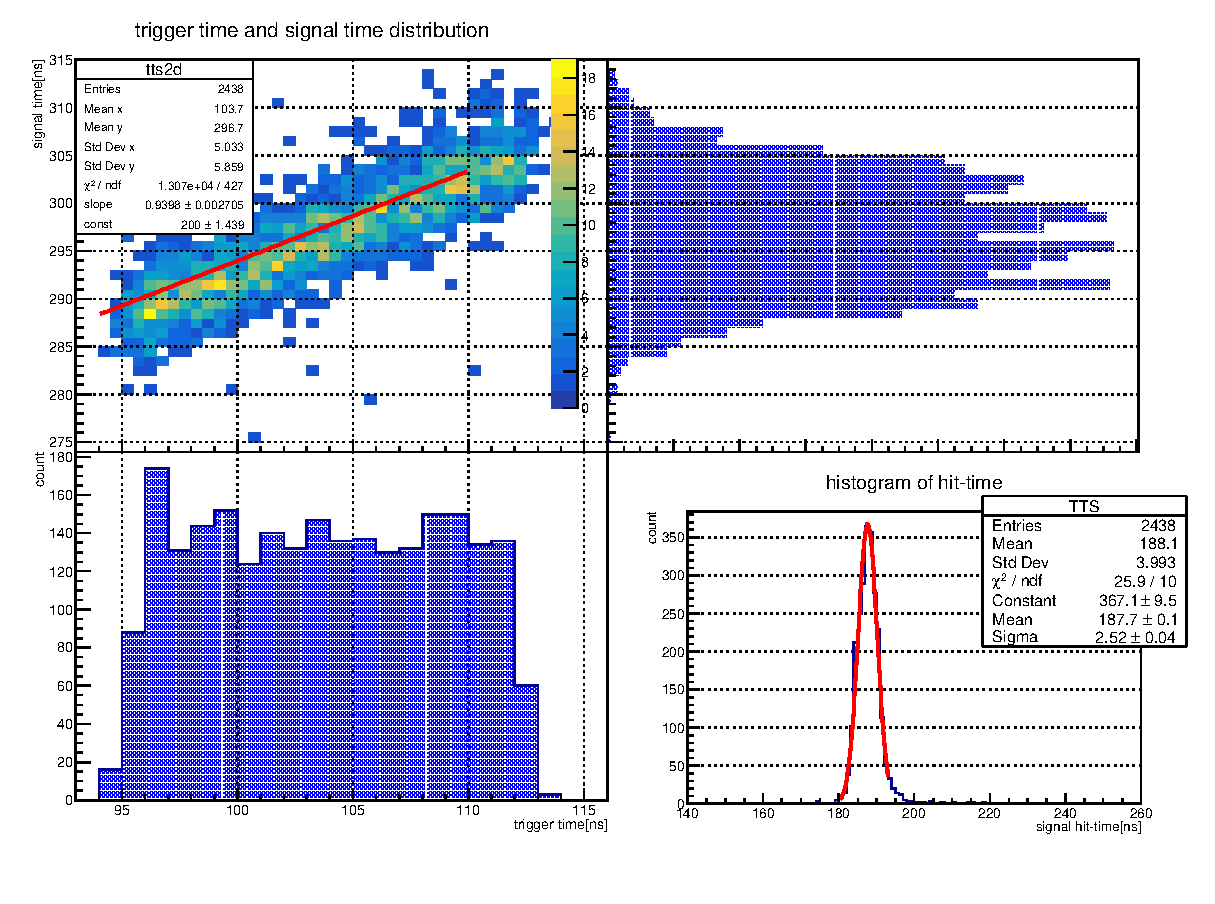
\includegraphics[width=0.74\textwidth]{ea0419-273} % 单图
\end{figure}
\end{frame}
%%%%%%%%%%%%%%%%%%%%%%%%%%%%%%%%%%%%%%%%%%%%%%%%%%%%%%%%%%%%%%%%
\begin{frame}{conclusion}
It seems that the hit-time distribution is drawer related.

\vspace{.5cm}
\hrule{}
\hrule{}
\vspace{.5cm}
Then I randomly selected several HAMAMATSU PMTS tested in drawer 113, their hit-time histograms all have "small foollowing peak"; While those PMTs tested in drawer 124 still only have one peak. 

\vspace{.5cm}
\hrule{}
\hrule{}
\vspace{.5cm}
\alert{So, it can be confirmed that the final hit-time distribution is drawer related rather than PMT related, and the measurement data need to be refined to meet our requirement.}
\end{frame}
%%%%%%%%%%%%%%%%%%%%%%%%%%%%%%%%%%%%%%%%%%%%%%%%%%%%%%%%%%%%%%%%
%%%%%%%%%%%%%%%%%%%%%%%%%%%%%%%%%%%%%%%%%%%%%%%%%%%%%%%%%%%%%%%%
\begin{frame}{MCP-PMT}
%\vspace{-1cm}
For MCP-PMT the hit-time distribution is quite bad.
\begin{figure}
\centering
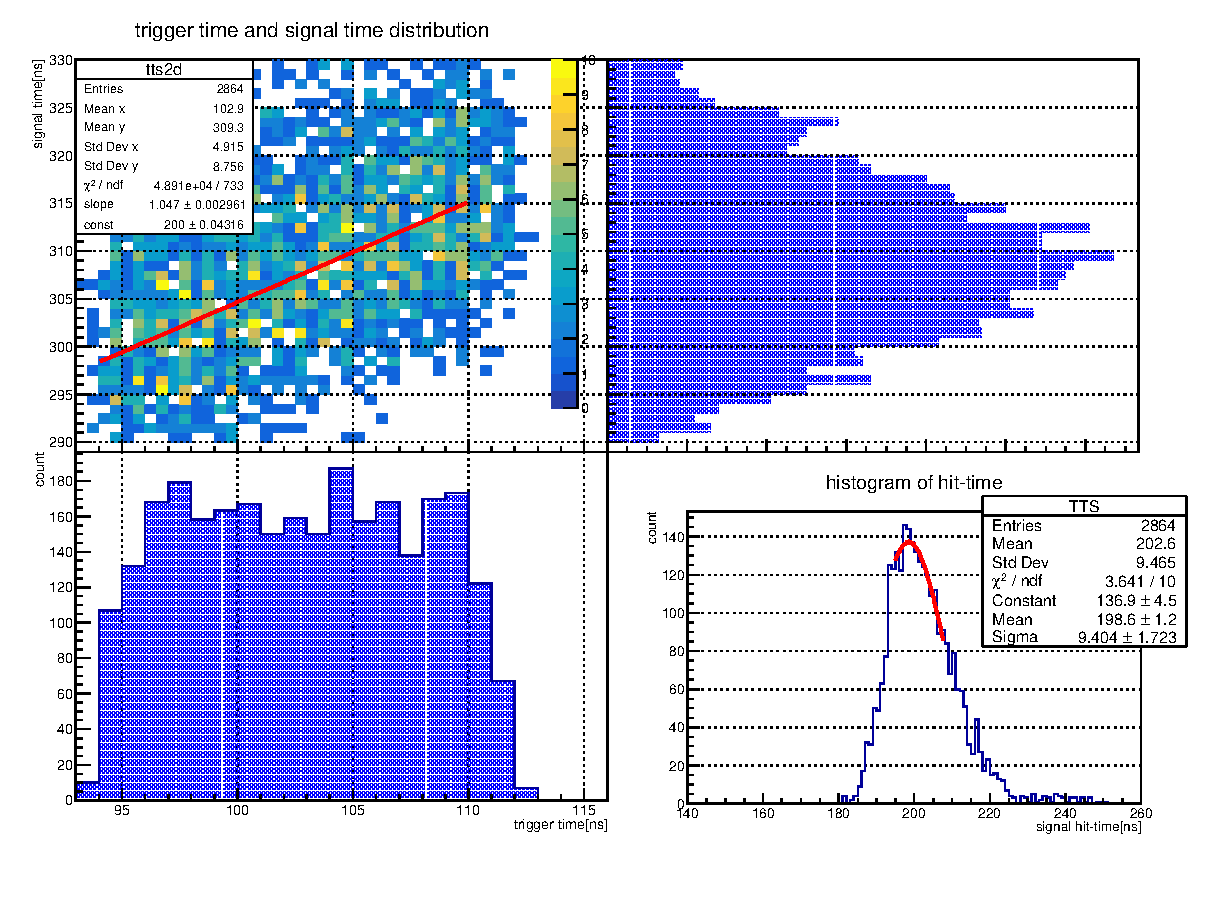
\includegraphics[width=0.7451\textwidth]{pa1703-1645} % 单图
\end{figure}
\end{frame}
\begin{frame}{discuss about the MCP results}
The data of this plot is from container 1, mass277, drawer 113, SN=PA1703-1645, MCP-PMT.\\
\vspace{.5cm}
\hrule{}
\hrule{}
\vspace{.5cm}
We can see from the above figure that:
\begin{itemize}
\item The PMT signal time is proportional to trigger time but worse than HAMAMATSU PMTs.
\item Trigger time also follow a uniform distribution 
\item PMT signal time, has a larger spread than HAMAMATSU PMTs.
\item In the 2-D histogram, the "small peak" in hit-time histogram become unclear but still recognizable.
\item Since the bad time performance of MCP tubes, they are not appropriate for system noise study.
\item The hittime of MCP PMT is slower($\sim $20ns) than HAMAMATSU PMT.
\end{itemize}
\end{frame}

\begin{frame}{improvements}
\begin{itemize}
\item Firstly, we need to evaluate the iternal time variation of electronics in each drawer.(one possible way is to replace the PMT output signal with corresponding synchronized TTS signal as the input of FADC).

\item Then, check and ensure the electronics time response meet our resolution requirement.

\end{itemize}
\end{frame}

\section{end}

\begin{frame}
\centering {\zihao{0} \color{red} \calligra{Thank You}}

\end{frame}


%\begin{frame}[allowframebreaks]
%\frametitle{References}
%\scriptsize
%\bibliographystyle{authordate1}
%\bibliography{R-GLMM-pkgs}
%\end{frame}

\appendix

\section*{附录}

%\begin{frame}{Softwares and Tools}

%\includegraphics[width=.2\textwidth]{software/r}\qquad
%\includegraphics[width=.16\textwidth]{software/stan} \\ 
%\includegraphics[width=.45\textwidth]{software/bioconductor}
%\includegraphics[width=.45\textwidth]{software/PyMC3} 

%\end{frame}
%% OpenBUGS  WinBUGS  JAGS
% library(R2OpenBUGS) # 2017-2-20 version 3.2-3.2
% library(R2WinBUGS) # 2015-07-29 version 2.1-21
% library(rjags) # 2016-02-19 version 4-6
% library(BRugs) # OpenBUGS 2017-06-26  version 0.9-0
% library(glmmBUGS) # Generalised Linear Mixed Models with BUGS and JAGS 2016-09-22 version 2.4.0
% library(R2jags) # Using R to Run 'JAGS'  2015-08-23	 version 0.5-7

% network
	% diagram DiagrammeR DiagrammeRsvg
 % library(help=graph)

 % library(help=Rgraphviz)
 % library(help=igraph)


%\begin{frame}{Ack}
%\begin{itemize}
%\item[\faGithub] \href{https://github.com/Cloud2016}{Cloud2016} \faAt Github
%\item[\aiOverleaf] \href{https://www.overleaf.com/}{Xiangyun} \faAt Overleaf
%\item[\aiarXiv] \href{https://arxiv.org/}{arXiv}
%\end{itemize}
%\end{frame}

\end{document} 


